\subsection{Transformada de Fourier em 2 dimensões}

A Transformada de Fourier em duas dimensões é uma extensão da Transformada de Fourier unidimensional, amplamente utilizada no processamento de sinais e imagens. Essa transformada permite converter um sinal definido no domínio espacial (como uma imagem, onde os pixels representam intensidades em coordenadas espaciais) para o domínio da frequência. No domínio da frequência, a transformada representa as componentes de frequência presentes na imagem, possibilitando a análise de características como padrões repetitivos, bordas e texturas.

A Transformada de Fourier bidimensional é definida matematicamente como:

$$
    F(u,v) = \sum_{x=0}^{N-1} \sum_{y=0}^{M-1} f(x,y) \cdot e^{-j 2\pi \left(\frac{ux}{N} + \frac{vy}{M}\right)},
$$

onde:
\begin{itemize}
    \item $f(x, y)$ representa a intensidade do pixel na posição $(x, y)$ no domínio espacial;
    \item $F(u, v)$ é o valor da Transformada de Fourier no ponto $(u, v)$ no domínio da frequência;
    \item $N$ e $M$ são as dimensões da imagem em pixels (largura e altura, respectivamente);
    \item $e^{-j 2\pi (\frac{ux}{N} + \frac{vy}{M})}$ é o fator de oscilação que determina como as frequências são calculadas.
\end{itemize}

Cada posição $(u, v)$ no espectro de frequência está associada a uma frequência radial, que pode ser calculada como:

$$
    D(u, v) = \sqrt{u^2 + v^2}.
$$

A frequência radial $D(u, v)$ está relacionada à distância do ponto $(u, v)$ em relação à origem do espectro de frequência, que corresponde à componente de frequência mais baixa (ou contínua) da imagem. As componentes de frequência mais altas, que correspondem a mudanças rápidas de intensidade na imagem (como bordas ou ruído), estão localizadas mais afastadas da origem no espectro.

A Transformada de Fourier bidimensional é amplamente utilizada em tarefas como filtragem no domínio da frequência, compressão de imagens, remoção de ruído e análise de padrões frequenciais, sendo uma ferramenta essencial no processamento de imagens digitais.

%%%%%%%%%%%%%%%%%%%%%%%%%%%%%%%%%%%%%%%%%%%%%%%%%%%%%%%%%%%%%%%%%%%%%%
\subsection{Audio}
De modo a realizar uma melhor comparação dos efeitos de filtragem de um áudio ruidoso, foram utilizados dois filtros distintos, ambos funcionando como passa-baixas. Esses filtros foram o \textit{Butterworth} e o \textit{Elíptico}.

Nessa seção serão apresentados cálculos de ordem e função de transferência de cada filtro utilizado.

\subsubsection{Filtro Butterworth}
Para que pudéssemos aplicar corretamente o filtro, foi necessário o cálculo da ordem do mesmo, bem como a atenuação da banda passante ($\epsilon$).

Foram definidos os seguintes parâmetros para o filtro \textit{Butterworth} passa-baixa:

\begin{enumerate}
    \item Banda passante $\omega_p=1000 \, \text{Hz}$
    \item Banda de rejeição $\omega_s = 2000\, \text{Hz}$
    \item Atenuação da banda passante $\alpha_p = 1dB$
    \item Atenuação da banda de rejeição $\alpha_s = 20dB$
\end{enumerate}


\subsubsection*{Executando o cálculo}
Incialmente, devemos realizar o cálculo da ordem do filtro, que segue a fórmula:

$$
    n = \left[ \frac{\log{\frac{10^{\alpha_s/10}- 1}{10^{\alpha_p/10}-1}}}{2\log{\omega_s/\omega_p}} \right]
$$

\begin{align} \
    n = \left[ \frac{\log{\frac{10^{20/10}- 1}{10^{1/10}-1}}}{2\log{(2\pi \cdot2000/2\pi\cdot 1000)}} \right] \\
    n = \left[ \frac{\log{\frac{100- 1}{1.25892541179-1}}}{2\log{2}} \right]                                  \\
    n = \left[ \frac{\log{382.349493298}}{0.60205999132} \right]                                              \\
    n = \left[ \frac{2.58246051898}{0.60205999132} \right]                                                    \\
    n = 4.28937407603                                                                                         \\
    \\
    \therefore n = 5
\end{align}


Em seguida, obtemos o valor de $A_{max}$ para calcular a função de transferência do filtro.

$$
    H(j\omega) = \frac{1}{\sqrt{1+\epsilon^2 \left( \frac{\omega}{\omega_p} \right)^{2n}}}
$$

Como na fórmula, é preciso o valor de $\epsilon$, que é calculado da seguinte forma:

$$
    \epsilon = \sqrt{10^{A_{max}/10}-1}
$$

Considerando que o nosso $A_{max}=1\, \text{dB}$, temos que:

\begin{align} \
    \epsilon = \sqrt{10^{1/10}-1}   \\
    \epsilon = \sqrt{0.25892541179} \\
    \therefore \epsilon = 0.509
\end{align}

Agora, aplicando o valor de $\epsilon$ e $n$ na fórmula da função de transferência, temos:

\begin{align} \
    H(j\omega) = \frac{1}{\sqrt{1 + 0.509^2 \left( \frac{\omega}{1000} \right)^{10}}} \\
    H(j\omega) = \frac{1}{\sqrt{1 + 0.259 \left( \frac{\omega}{1000} \right)^{10}}}
\end{align}


\subsubsection{Filtro Elíptico}
Para que pudéssemos aplicar corretamente o filtro, foi necessário o cálculo da ordem do mesmo, bem como a atenuação da banda passante ($\epsilon$).

Foram definidos os seguintes parâmetros para o filtro \textit{Elíptico} passa-baixa:

\begin{enumerate}
    \item Banda passante $\omega_p=1000 \, \text{Hz}$
    \item Banda de rejeição $\omega_s = 2000\, \text{Hz}$
    \item Atenuação da banda passante $\alpha_p = 1dB$
    \item Atenuação da banda de rejeição $\alpha_s = 60dB$
\end{enumerate}


\subsubsection*{Executando o cálculo da ordem do filtro}
Incialmente, devemos realizar o cálculo da ordem do filtro, que segue a fórmula:

\begin{align} \
    k = \frac{\omega_p}{\omega_s}                           \\
    u = \frac{1 - \sqrt[4]{1 - k^2}}{2 (1+\sqrt[4]{1-k^2})} \\
    q = u + 2u^5 + 15u^9 + 150u^13                          \\
    D = \frac{10^{\alpha_s/10} - 1}{10^{\alpha_p/10}-1}     \\
    n = \text{ceil} \left( \frac{\log{16D}}{\log{1/q}} \right)
\end{align}

Substituindo e encontrando os valores, temos:

\begin{align*} \
    k = \frac{\omega_p}{\omega_s} \\
    k = \frac{1000}{2000}         \\
    \therefore k = 0.5
\end{align*}

Tendo o valor de $k$, podemos calcular $u$:

\begin{align*} \
    u = \frac{1 - \sqrt[4]{1 - k^2}}{2 (1 + \sqrt[4]{1 - k^2})}     \\
    u = \frac{1 - \sqrt[4]{1 - 0.5^2}}{2 (1 + \sqrt[4]{1 - 0.5^2})} \\
    \\
    u = \frac{1 - 0.9306}{2 (1 + 0.9306)}                           \\
    u = \frac{0.0694}{3.8612}                                       \\
    u =\approx 0.01797
\end{align*}

Com o valor de $u$, calcula-se $q$:

\begin{align*}
    q = u + 2u^5 + 15u^9 + 150u^{13}                                                     \\
    q = 0.01797 + 2(0.01797)^5                                                           \\
    \quad + 15(0.01797)^9 + 150(0.01797)^{13}                                            \\
    \\
    q = 0.01797 + 2 \cdot (1.8790937 \times 10^{-9})                                     \\
    \quad + 15 \cdot (1.9638449 \times 10^{-16}) + 150 \cdot (2.0524186 \times 10^{-23}) \\
    \\
    q = 0.01797 + 3.7581874 \times 10^{-9}                                               \\
    \quad + 2.9457674 \times 10^{-15} + 3.0786279 \times 10^{-21}                        \\
    \\
    q \approx 0.017970003758190345
\end{align*}


Como os termos menores são extremamente pequenos, podemos considerar $q=u$ no cálculo final de $n$.
Porém antes de calcular $n$, devemos encontrar $D$:

\begin{align*} \
    D = \frac{10^{\alpha_s / 10} - 1}{10^{\alpha_p / 10} - 1} \\
    D = \frac{10^{60 / 10} - 1}{10^{1 / 10} - 1}              \\
    D = \frac{10^{6} - 1}{1.25892541179 - 1}                  \\
    D = \frac{999999}{0.25892541179}                          \\
    D \approx 3862112.23
\end{align*}

Por fim, temos que:

\begin{align*} \
    n = \text{ceil} \left( \frac{\log{16D}}{\log{1/q}} \right)                                    \\
    n = \text{ceil} \left( \frac{\log{16 \cdot 3862112.23}}{\log{1/0.017970003758190345}} \right) \\
    n = \text{ceil} \left( \frac{7.79094487255}{1.74545183206} \right)                            \\
    n = \text{ceil} \left( \frac{7.79094487255}{1.74545183206} \right)                            \\
    n = \text{ceil} (4.4635691054)                                                                \\
    \therefore n = 5
\end{align*}

Portanto, é possível definir que o filtro elíptico aplicado terá \textbf{ordem 5}.


\subsubsection*{Cálculo da função de transferência}

Agora que temos a ordem $n = 5$, podemos expressar a função de transferência $H(s)$ para o filtro elíptico passa-baixa.

A forma geral da função de transferência para um filtro elíptico passa-baixa é:

$$
    H(s) = \frac{\prod_{k=1}^{N} (s - z_k)}{\prod_{k=1}^{M} (s - p_k)} \cdot \text{Ganho}
$$

onde:
\begin{enumerate}
    \item $N$ é o número de zeros,
    \item $M$ é o número de polos (5 neste caso),
    \item $z_k$ são os zeros da função de transferência,
    \item $p_k$ são os polos da função de transferência.
\end{enumerate}

\begin{lstlisting}[language=Octave]
% n = ordem, Rp = ripple na banda passante (em dB)
% Rs = atenuacao na banda de parada (em dB)
% Wp = frequencia de corte normalizada
% 'low' indica filtro passa-baixa
[b, a] = ellip(n, Rp, Rs, Wp, 'low');

% (z) zeros, (p) polos e (k) ganho
[z, p, k] = tf2zp(b, a);
figure;
zplane(z, p);  % Plot
title('Polos e Zeros do Filtro Eliptico');
\end{lstlisting}

A execução do código apresentado permitiu a obtenção dos zeros, polos e do ganho do filtro elíptico, que são elementos fundamentais para a análise e caracterização da sua função de transferência. A Figura \ref{fig:elliptic_zeros_and_poles} apresenta a distribuição dos zeros e polos no plano complexo, destacando a sua relação com as propriedades do filtro.

\begin{figure}[H]
    \centering
    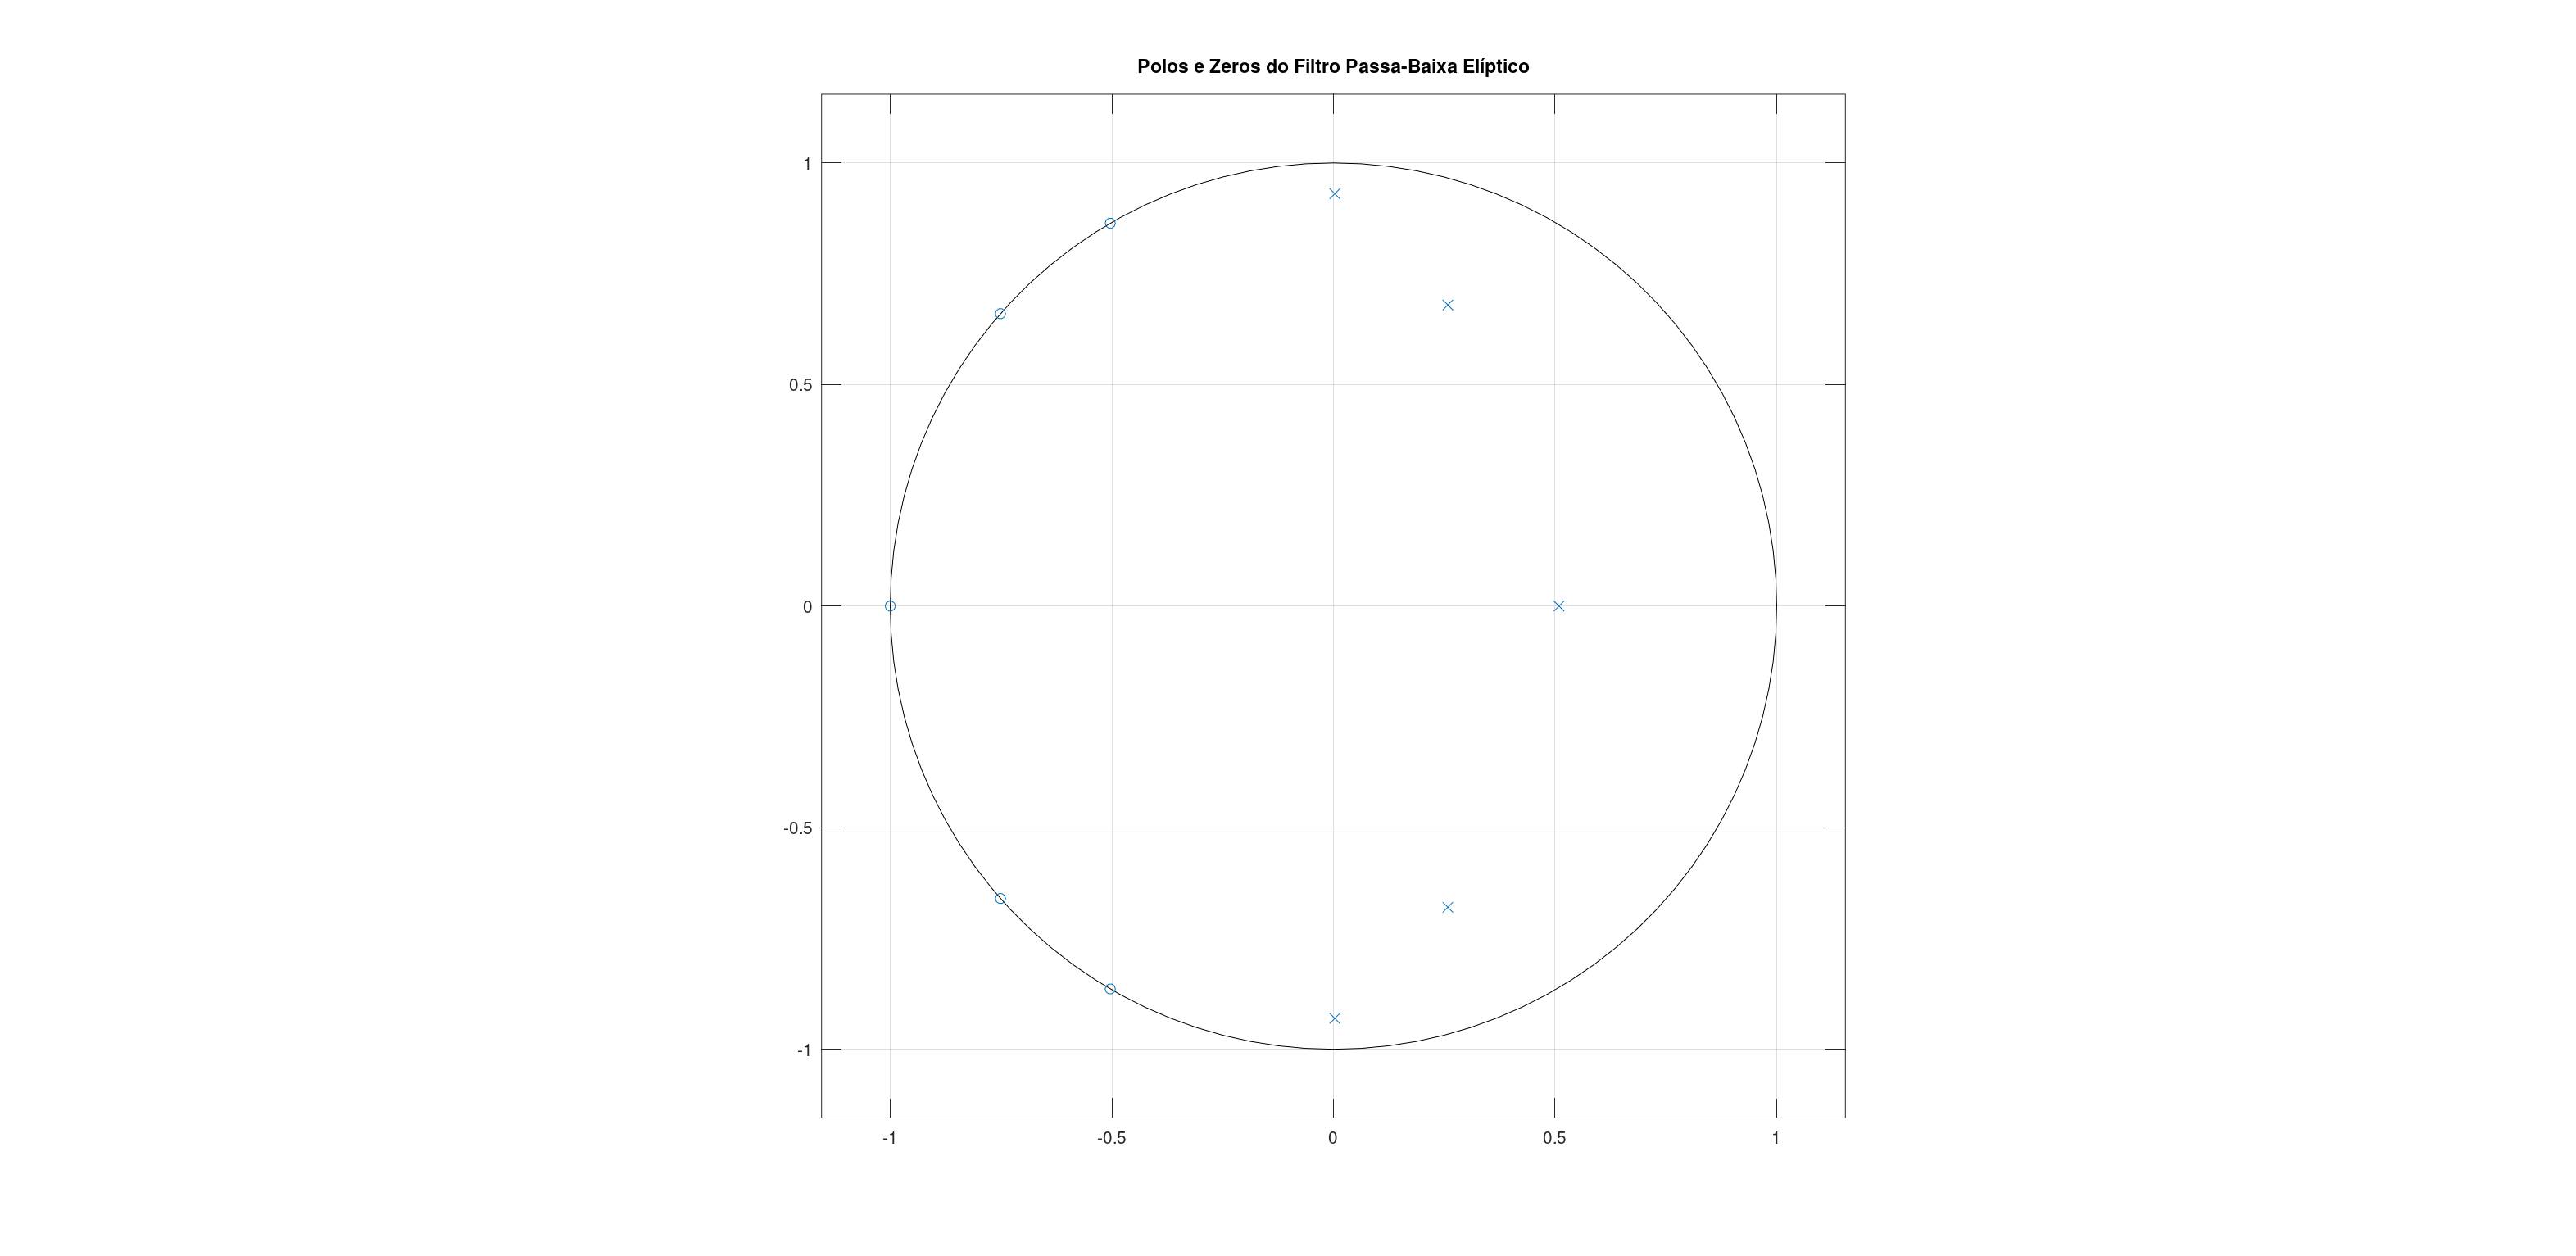
\includegraphics[width=1\linewidth]{02_analytic_development/assets/elliptic_zeroes_and_poles.png}
    \caption{Zeros, polos e ganho obtidos a partir da execução do código do filtro elíptico.}
    \label{fig:elliptic_zeros_and_poles}
\end{figure}

Portanto a função de transferência final do filtro é:
\begin{align*}
    H(s) = \frac{(s + 1)(s + 0.5037 - 0.8639i)}{(s - 0.0030 - 0.9304i)(s - 0.0030 + 0.9304i)}                     \\
    \quad \cdot \frac{(s + 0.5037 + 0.8639i)(s + 0.7514 - 0.6599i)}{(s - 0.2580 - 0.6795i)(s - 0.2580 + 0.6795i)} \\
    \quad \cdot \frac{(s + 0.7514 + 0.6599i)}{(s - 0.5088)}                                                       \\
    \quad \cdot 0.043890
\end{align*}


%%%%%%%%%%%%%%%%%%%%%%%%%%%%%%%%%%%%%%%%%%%%%%%%%%%%%%%%%%%%%%%%%%%%%%
\subsection{Imagem}


\subsubsection{Filtro Chebyshev}
Para que pudéssemos aplicar corretamente o filtro, foi necessário o cálculo da ordem do mesmo.

Foram definidos os seguintes parâmetros para o filtro \textit{Chebyshev} rejeita-faixa:

\begin{enumerate}
    \item Banda passante $\omega_p= [98, 102] \, \text{Hz}$
    \item Banda de rejeição $\omega_s = [99, 101]\, \text{Hz}$
    \item Atenuação da banda passante $\alpha_p = 1dB$
    \item Atenuação da banda de rejeição $\alpha_s = 60dB$
\end{enumerate}


\subsubsection*{Executando o cálculo}
Incialmente, devemos realizar o cálculo da ordem do filtro, que segue a fórmula:

$$
    n = \text{ceil} \left[ \frac{\cosh^{-1}{\sqrt{\frac{10^{\alpha_s/10}- 1}{10^{\alpha_p/10}-1}}}}{\cosh^{-1}{\omega_s/\omega_p}} \right]
$$


Como as bandas de passante e rejeição são dadas como intervalos, devemos usar a frequência central de cada intervalo.

\subsubsection*{Calculando o denominador}

Quando as frequências são fornecidas em Hertz (Hz), elas precisam ser normalizadas em relação à frequência de Nyquist. A frequência de Nyquist é dada por $f_{\text{Nyquist}} = \frac{f_s}{2}$, onde $f_s$ é a taxa de amostragem.

Neste caso, a taxa de amostragem $f_s$ é 256 Hz. Então, as frequências passante ($\omega_p$) e rejeição ($\omega_s$) precisam ser ajustadas dividindo cada valor pela frequência de Nyquist.

A fórmula para normalizar as frequências $\omega_p$ e $\omega_s$ é:

\begin{align*} \
    \omega_p = \frac{\text{Freqüência de passante}}{128}                       \\
    \omega_s = \frac{\text{Freqüência de rejeição}}{128}                       \\
    \\
    \text{Substituindo os valores}                                             \\
    \\
    \omega_p = \left[\frac{98}{128}, \frac{102}{128}\right] = [0.7656, 0.7969] \\
    \omega_s = \left[\frac{99}{128}, \frac{101}{128}\right] = [0.7734, 0.7891]
\end{align*}

Em seguida, aplicamos a transformação tangente para essas frequências normalizadas, utilizando a seguinte fórmula:

\begin{align*} \
    \text{passb} = \tan\left(\frac{\pi \cdot \omega_p}{2}\right)         \\
    \text{stopb} = \tan\left(\frac{\pi \cdot \omega_s}{2}\right)         \\
    \\
    \text{Aplicando a transformação tangente}                            \\
    \\
    \text{passb} = \tan\left(\frac{\pi \cdot [0.7656, 0.7969]}{2}\right) \\ \quad \Rightarrow \quad \text{passb} = [2.592099, 3.027442] \\
    \text{stopb} = \tan\left(\frac{\pi \cdot [0.7734, 0.7891]}{2}\right) \\ \quad \Rightarrow \quad \text{stopb} = [2.689781, 2.907342]
\end{align*}


Com as frequências passante ($\text{passb}$) e rejeição ($\text{stopb}$) transformadas, podemos calcular o valor de $\text{freqRatio}$ usando a fórmula:

$$
    \text{freqRatio} = \text{min}_{\text{absoluto}} \left(\frac{\text{stopb} \cdot (\text{passb}[1] - \text{passb}[2])}{\text{stopb}^2 - \text{passb}[1] \cdot \text{passb}[2]} \right)
$$

Substituindo os valores:

\begin{align*} \
    \text{freqRatio} = \frac{\{2.689781, 2.907342\} \cdot (2.592099 - 3.027442)}{\{2.689781, 2.907342\}^2 - 2.592099 \cdot 3.027442} \\
    \text{freqRatio} = \frac{\{2.689781, 2.907342\} \cdot (-0.4346)}{\{7.2392, 8.4526\} - 7.8541}                      \\
    \\
    \begin{array}{cc}
\text{freqRatio} = \frac{-1.1700}{-0.6149} & \text{freqRatio} = \frac{-1.2635}{0.5985} \\
\text{freqRatio} = 1.9027                  & \text{freqRatio} = -2.1111
\end{array}
\\
\therefore \text{freqRatio} = 1.9027
\end{align*}

Este é o valor de $\text{freqRatio}$ calculado a partir das frequências normalizadas e transformadas.

Agora, vamos substituir os valores conhecidos na fórmula para calcular a ordem do filtro:

\begin{align*} \
    n = \text{ceil} \left[ \frac{\cosh^{-1}{\sqrt{\frac{10^{60/10}- 1}{10^{1/10}-1}}}}{\cosh^{-1}{freqRatio}} \right] \\
    n = \text{ceil} \left[ \frac{\cosh^{-1}{\sqrt{\frac{999999}{0.2589}}}}{\cosh^{-1}{freqRatio}} \right]            \\
    n = \text{ceil} \left[ \frac{\cosh^{-1}{\sqrt{3862491.30939}}}{\cosh^{-1}{1.9027}} \right]                           \\
    n = \text{ceil} \left[ \frac{\cosh^{-1}{1965.3222}}{\cosh^{-1}{1.9027}} \right]                                  \\n = \text{ceil} \left[ \frac{8.27656}{1.2589} \right]                                     \\
    n = \text{ceil} [6.5744]                                                                                      \\
    \therefore n = 7
\end{align*}


\subsubsection{Filtro Butterworth: rejeita-faixa}
Foram definidos os seguintes parâmetros para o filtro \textit{Butterworth} rejeita-faixa:

\begin{itemize}
    \item Frequências de passagem: $f_p = [98, 106] \, \text{Hz}$;
    \item Frequências de rejeição: $f_s = [99, 101] \, \text{Hz}$;
    \item Ondulação na banda de passagem: $R_p = 0.1 \, \text{dB}$;
    \item Atenuação mínima na banda de rejeição: $R_s = 20 \, \text{dB}$;
    \item Frequência de amostragem: $F_s = 256 \, \text{Hz}$.
\end{itemize}

\subsubsection*{Cálculo da Ordem}
Seguindo a \textbf{Equação ~\ref{eq:butterworth_n_formula}} definida previamente, podemos realizar os cálculos da ordem:

\begin{align*} \
    n = \left[ \frac{\log{\frac{10^{20/10}- 1}{10^{10^{-2}}-1}}}{2\log{(\text{freqRatio})}} \right] \\
    %n = \left[ \frac{\log{\frac{100- 1}{1.02329299228-1}}}{2\log{(\text{freqRatio})}} \right]                                  \\
    n = \left[ \frac{\log{\frac{99}{0.02329299228}}}{2\log{1.9525}} \right]                         \\
    %n = \left[ \frac{\log{4250.2053}}{2\log{1.9525}} \right]                                                    \\
    n = \left[ \frac{3.6284}{0.58118} \right]                                                       \\
    n = 6.243                                                                                       \\
    \\
    \therefore n = 7
\end{align*}

